\section{The \ouralg~algorithm}
\label{sec:ouralg}
The main idea of our approach is to exploit the well-known mathematical fact that, for any smooth maps $f,g,h$ with
$f =h\circ g$, the differentials $Df,Dh,Dg$ at any point are in
the {\em linear} relationship $Df = Dh Dg$. 
Thus, given sets of functions $\phi_{1:m}$ and $g_{1:p}$ of a smooth manifold $\M$, we propose to recover a subset $g_{S}$ of $g_{1:p}  $ such that $\phi_{1:m} =h \circ g_S$ by solving a set of dependent linear sparse recovery problems.
Note that there is one problem for each data point, and the support is selected without explicit estimation of $h$.

The \ouralg~algorithm, the main algorithm of this paper, implements this idea.
It takes as input data $\dataset$ sampled from an unknown manifold $\M$, a dictionary $\G  = g_{1:p}$ of functions defined on $\M$ (or alternatively on an open subset of the ambient space $\rrr^D$ that contains $\M$), and an embedding $\phi(\dataset)$ in
$\rrr^m$.
The output of \ouralg~is a set $S$ of indices in $\G$,
representing the functions in $\G$ that explain $\M$. 

The first part of the algorithm calculates the necessary gradients.
This comprises Steps \ref{alg:neb}--\ref{alg:prob} and is detailed in Sections \ref{sec:grad-g} and \ref{sec:pull-back}.
For each data point, we perform several operations in the tangent subspaces $\T_{\xi_i}\M$ and $\T_{\phi(\xi_i)} \phi (\M)$.
We thus estimate orthonormal bases $T_i^\M$ and $T_i^\phi$ of these spaces using \ref{alg:tan} and \rmalg.  
Steps \ref{alg:neb} and \ref{alg:lap} consist of constructing the neighborhood graph and the kernel and Laplacian matrices that we use to compute these tangent spaces.
The gradients of the dictionary w.r.t. the manifold $\M$ are then obtained as columns of the $d\times p$ matrices $X_i$ in Steps \ref{alg:dict} and \ref{alg:dict_proj} as described in Section \ref{sec:grad-g}.
Finally, the gradients at $\xi_i$ of the coordinates $\phi_{1:m}$, also seen as functions of $\M$, are calculated as columns of the $d \times m $ matrix $Y_i$ by the \dpullalg~algorithm in Step \ref{alg:pb} as described in Section \ref{sec:pull-back}. 
%These operations are described in Section \ref{sec:grad-g}.

The second part of the algorithm, namely Step \ref{alg:glasso}, finds the support $S$ by solving a sparse regression problem; this is described in Section \ref{sec:flasso-manifold}.
In this step, a \flassoalg~algorithm is called to perform sparse regression of the manifold coordinates' gradients $Y_{1:n}$ on the gradients of the dictionary functions $X_{1:n}$.
The indices of those dictionary functions whose $\beta$ coefficients are not identically null represent the support set $\supp \beta$.
%The following section presents the main steps of the algorithm, including formal definitions of the relevant gradients.

There are several optional steps and substitutions in our algorithm.
An embedding can be computed in Step \ref{alg:embed}, or input separately by the user.
We denote this step generically as \embedalg.
Furthermore, although we explicitly describe tangent space estimation methods of both $\T_{\xi_i} \M$ and $\T_{\phi(\xi_i)} \phi (\M)$ in our algorithms, other approaches may be used as well.
Finally, scaling of functions is addressed through normalization in Section \ref{sec:ouralg-normalization}.
%In step \ref{alg:tan}, orthogonal bases of these tangent subspace are estimated by the \tppalg~algorithm described in Section \ref{sec:background}.

%
\begin{algorithm}[H]
\floatname{algorithm}{\ouralg}
\renewcommand{\thealgorithm}{}
\caption{(Dataset $\dataset$, dictionary $\G$, embedding coordinates $\phi(\dataset)$,  intrinsic dimension $d$, kernel bandwidth $\epsilon_N$, neighborhood cutoff size $r_N$, regularization parameter $\lambda$)}
\begin{algorithmic}[1]
\STATE Construct $\neigh_i$ for $i=1:n$; $i'\in \neigh_i$ iff $||\xi_{i'}-\xi_{i}||\leq r_N$, and local data matrices $\Xi_{1:n}$ \label{alg:neb}
\STATE Construct kernel matrix and Laplacian $K, L\,\gets\,$\lapalg($\neigh_{1:n},\Xi_{1:n},\epsilon_N$) \label{alg:lap}
\STATE [Optionally compute embedding: $\phi(\xi_{1:n})\gets$\embedalg$(\dataset,\neigh_{1:n},m,\ldots)$] \label{alg:embed}
  \FOR {$i=1,2,\ldots n$ (or subset) {\em (Prepare gradients for group lasso)}} 
  \STATE Compute basis  ${T_i^\M} \gets $\tppalg$(\Xi_i, K_{i, \neigh_i},d)$ \label{alg:tan}
  \STATE Compute $\nabla_\xi g_j (\xi_i)$ for $j=1,\ldots p$ \label{alg:dict}
  \STATE Project $X_i\gets {T_i^\M}^T\nabla_\xi g_{1:p}$ \label{alg:dict_proj}
  \STATE Compute $Y_i \gets$\dpullalg$(\Xi_i, \Phi_{i},T_i^\M,  L_{i, \neigh_i},  d)$ \label{alg:pb} \label{alg:prob}
  \ENDFOR
\STATE $\beta\,\gets$ \flassoalg$(X_{1:n}, Y_{1:n}, \lambda/\sqrt{mn})$ \label{alg:glasso}
\STATE {\bf Output} $S=\supp \beta$ 
\end{algorithmic}
\end{algorithm}

\subsection{Gradients and coordinate systems}
\label{sec:explain-dphi}

The \ouralg~algorithm regresses the gradients of the coordinate
functions $\phi_{1},\ldots \phi_m$ on the
gradients of the dictionary functions.
Both sets of gradients are with respect to the manifold $\M$, and so this requires calculating or estimating various gradients in the
same $d$-dimensional coordinate system.
This and the following two sections explain these procedures. 

First, note that by assumption we have two Euclidean spaces $\rrr^D$ and $\rrr^m$, in which manifolds $\M$ and $\phi(\M)$ of dimension $d$ are embedded.
Denote gradients w.r.t. the Euclidean coordinate systems in $\rrr^D$ and $\rrr^m$ by $\nabla_\xi$ and $\nabla_\phi$, respectively.
Since our interest is in functions on manifolds, we
also define the gradient of a function on a manifold $\M$.
The {\em gradient} of $f$ at $\xi$, denoted $\grad_{\M} f(\xi)\in\T_\xi\M$, is defined by $\langle \grad_{\M} f(\xi),v\rangle=Df(\xi)v$ for any $v\in \T_\xi \M$.
Denote gradients in the tangent bundles of $\M$ and $\phi(\M)$ by $\grad_\M$ and $\grad_{\phi(\M)}$, respectively. 
For each data point $\xi_i$, we will fix bases $T_i^\M$ in $\T_{\xi_i}\M$ and $T_i^\phi$ in $\T_{\phi (\xi_i)} \phi (\M)$.
Gradients expressed in these coordinate systems will be denoted by $\grad_{T_i^\M}$ and $\grad_{T_i^\phi}$ respectively.
The next section describes how to calculate dictionary gradients in the bases $T_i^\M,\,i\in[n]$.

\subsection{Calculating the gradients of the dictionary functions}
\label{sec:grad-g}

Our goal is to obtain $X_i$, the matrix containing $\grad_{T_i} g_j (\xi_i)$ as columns, where $g_j$ is a function in the dictionary $\G$.
By definition, for any basis $T_i^\M \in \rrr^{D\times d}$ of $\T_{\xi_i}\M$,
\beq
\label{eq:gradprojg} \grad_{T_i^\M}g_j(\xi_i)\;=\;T_i^T\nabla_{\xi}g_j(\xi_i).
\eeq
In other words, $\grad_{T_i^\M}g_j$ is the projection of $\nabla_\xi g_j$ on the basis $T_i^\M$.
These bases of $\T_{\xi_i}\M$, for every $i$, are estimated by \tppalg~as described in Section \ref{sec:background}.
The gradients $\nabla_\xi g_j(\xi_i)$ are known analytically, by assumption.
We thus construct matrices $X_i$, for $i=1,\ldots n$, with $p$ columns representing the gradients of the $p$ dictionary functions;
%
\beq \label{eq:X-manifold}
X_i\,=\,[\grad_{T_i^\M} g_j(\xi_i)]_{j=1:p}\,\in \rrr^{d\times p}.
\eeq
Next, we explain our estimator of $\grad_{T_i^\M} \phi_k$, the gradients of the coordinate functions.

\subsection{Estimating the coordinate gradients by pull-back}
\label{sec:pull-back}

Our goal is to obtain $Y_i$, the matrix containing $\grad_{T_i^\M}\phi_k (\xi_i)$ as columns.
Since $\phi$ is implicitly determined by a manifold embedding algorithm, the gradients of $\phi_k$ are often not analytically available, and $\phi_k$ is known only through its values at the data points.
We therefore introduce a gradient estimator based on the notion of vector-pullback between tangent spaces.

The \dpullalg~Algorithm performs gradient estimation via local linear regression in tangent spaces $\T \M$ and $\T \phi(\M)$.
%\comment{We therefore estimate these gradients by in order to define a pullback between the tangent spaces $\T \M$ and $\T \phi \M$ \cite{Luo2009-mp} \cite{2013arXiv1305.7255P}.} 
This algorithm takes as inputs the local neighborhoods $\Xi_i$ and $\Phi_i$ of points $\xi_i$ and $\phi_i$ in the original and embedding spaces, respectively, as well as bases $T_i^\M$ of $\T_{\xi_i}\M$ and $T_i^\phi$ of $\T_{\phi_i} \M$.
Estimation of $T_i^\M$ is accomplished as in the previous section, while $T_i^\phi$ is estimated via the singular vectors output by \rmalg~ \citep{2013arXiv1305.7255P} described in Section \ref{sec:background}.
%Note that both of these tangent space estimators take as input the row of the Laplacian matrix corresponding to $i$.  
Geometrically, at each data point, this algorithm first projects gradients of the coordinate functions $\nabla_{\phi} \phi_k$ onto $T_{\phi(\xi_i)} \phi(M)$ to get $\grad_{T_i^\phi} \phi_k$, and then pulls these back to $T_i^\M$ to get $\grad_{T_i^\M} \phi_k$ by solving a linear system with respect to the neighborhood.
%The idea of the algorithm is to use this correspondence in order to pull back the gradient of the coordinate function $\phi_k$ into the coordinates $T_i$.

%We , and introduce an algorithm that estimates the gradient through projection onto 

This algorithm is based on the observation that gradient estimation on a manifold is exactly the operation of vector projection and pullback between tangent spaces of isometric Riemannian manifolds.
% following observation about gradients in coordinate systems with metric.
To see this, note that in a coordinate system $T_i^\phi$, writing $\g$ in $T_i^\phi$ as $G$, we have the definition
\beq
\grad_{T_i^\phi, G} f = G^{-1} \grad_{T_i^\phi, I_d} f
\eeq
where $\grad_{T_i^\phi, I_d} f =\grad_{T_i^\phi} f =  {T_i^\phi}^T \nabla_\phi f$ is with respect to the identity metric in $\rrr^m$ \citep{Lee:03}.
Thus, since $\grad_{\phi(\M)} \phi_k \in \tphim$, by the definition of $\g$  \eqref{eq:rmetric0}, we have that
%$( \Xi_i {T_i^\M} )^T  Y_i \,=\,   \Phi_i {T_i^\phi} $ 
\beq%\label{eq:gref-diff}
(D \phi^{-1} u)^T   \grad_{T_i^\M} \phi_k  \,\approx\, u^T \grad_{T_i^\phi, I_d} \phi_k \,\quad {i'\in \neigh_i}
\eeq
where $u \in \tphim$.
In particular, note that this is invariant to $\g$.
Hence, since $T_i^\M$ and $T_i^\phi(M)$ approximate the logarithmic map to the first order with error tending to 0 within the neighborhood radius \citep{coifman:06}, we have that
\beq\label{eq:gref-diff}
((\xi_{i'}-\xi_i)^T T_i^\M)^T Y_i \,\approx\, ( \phi(\xi_{i'})-\phi(\xi_i))^T T_i^\phi \,\quad {i'\in \neigh_i}
\eeq
with
\beq \label{eq:yYbetaijk-manifold}
Y_i\,=\,[y_{ik}]_{k=1}^m\,=\,[\grad_{T_i}\phi_k(\xi_i)]_{k=1}^m\in \rrr^{d\times m}.
\eeq

As long as sufficient neighbors are present, $A$ can be made of full rank $d$, and we can obtain $Y_i$ as the least-squares solution of 
\beq\label{eq:yi-manifold2}
(\Xi_i^T T_i^\M)^T Y_i \,\approx\,  \Phi_i T_i^\phi \,\quad {i'\in \neigh_i}.
\eeq

From a statistical perspective, this method is exactly local multivariate multiple linear regression with projection onto the manifolds $\M$ and $\phi(\M)$; it is local principal components regression with the additional step of projection onto the manifold in in the embedding coordinates.
It provides an alternative approach to regularized methods such as \citet{Aswani2011-li}
 for encouraging robustness to both statistical noise around $\M$ and $\phi(\M)$ and lowering the effective dimensionality of the regression problem.
Finally, note that when $m=d$, assuming a good embedding, then $T_i^\phi = I_d$.

\begin{algorithm}[H]
\floatname{algorithm}{\dpullalg}
\renewcommand{\thealgorithm}{}
\label{alg:pullback} 
\caption{local data $\Xi_i$, local embedding coordinates $\Phi_{i}$ basis $T_i^\M$ (Optional: $T_i^\phi$ or Laplacian row $L_{i,\neigh_i}$, intrinsic dimension $d$)}
\begin{algorithmic}[1]
%  \STATE {\bf Input} .
\STATE Compute tangent space $T_i^\M \gets$ \tppalg$(( L_{i,\neigh_i}, \Xi_{i}, d)$ (Optional import).
%\STATE Compute tangent space $T_i^\phi \gets \svd (\rmalg(( L_{i,\neigh_i}, \Phi_{i}, d),d)$
  \STATE Compute pushforward metric $G_i\gets$ \rmalg$( L_{i,\neigh_i}, \Phi_{i}, d)$ (Optional import $T_i^\phi$).
  \STATE Compute $T_i^\phi, \Lambda_i= \svd(G_i, d)$. (Optional import $T_i^\phi$).
   %\STATE Project $A_i=T_i^T(\Xi_i-\xi_i\bm{1}_{k_i}^T)$.
   %\STATE Compute $B_i = \Phi_{i} - \phi(\xi_i)\bm{1}_{k_i}^T  \in\rrr^{|\neigh_i| \times m }$.
   \STATE Solve linear system $( \Xi_i {T_i^\M} )^T  Y_i \,=\,   \Phi_i {T_i^\phi} $ as in \eqref{eq:yi-manifold2}
  \STATE {\bf Output} $Y_i$ 
%  \eqref{eq:pullbacksystem}
\end{algorithmic}
\end{algorithm}

%The columns of $A_i$ and $Y_i$ are vectors in $\T_{\xi_i}\M$, the columns of $B_i$ are in $\rrr^m$ and the columns of $\tilde{B}_i$ are in $\T_{\phi(\xi_i)}\phi(\M)$.

%Of these matrices, $A_i$ and $B_i$ can be easily computed (Steps 2 and 3 of Algorithm \dpullalg), while $Y_i$ contains the gradients we want to estimate. Note that when $m=d$, $B_i=\tilde{B}_i$. These vectors are shown schematically in Figure \ref{fig:pullback}.
%where 
%\beq
%A_i\,=\,\left[{T_i^\M}^T (\xi_{i'}-\xi_i)\right]_{i'\in
 % \neigh_i} \in \rrr^{d\times k_i} ,
%B_i\,=\,\left[{T_i^\phi(M)}^T \phi(M)} \phi(\xi_{i'})-\phi(\xi_i)\right]_{i'\in \neigh_i}
%\;\in \rrr^{m\times k_i},
%\eeq
%This is a dimension-reduced adaptation of the usual linear regression formula.
%All three steps depend on the the pushforward Riemannian metric $G_i$ associated with the tangent subspace $\T_{\phi(\xi_i)}\phi(\M)$. This is estimated  using the \rmalg~algorithm  \citep{2013arXiv1305.7255P} described in Section \ref{sec:background}. For each $i$, $G_i$ is the associated push-forward Riemannian metric at $\phi(\xi_i)$,  expressed in the coordinates of $\rrr^m$ by $G_i$. This is done in Step 1 of the \dpullalg~Algorithm.

%Instead of estimating these gradients naively from differences $\phi_k(\xi_i)-\phi_k(\xi_{i'})$ between neighboring points, we first estimate their values in $\T_{\phi(\xi_i)}\phi(\M)$, then use the differential geometric notion of vector {\em pull back} to obtain them in the $T_i$ coordinate system.
%This method is novel, and is of independent interest as it allows tranformations of vector fields between non-isometric embeddings of the data. 

%We make the following notations, with $\proj_T v$ denoting the Euclidean projection of vector $v$ onto subspace $T$.
% 
%\beq
%A_i\,=\,\left[\proj_{\T_{\xi_i}\M}(\xi_{i'}-\xi_i)\right]_{i'\in
%  \neigh_i} \in \rrr^{d\times k_i} 
%\eeq
%
%\beq \label{eq:yYbetaijk-manifold}
%Y_i\,=\,[y_{ik}]_{k=1}^m\,=\,[\grad_{T_i}\phi_k(\xi_i)]_{k=1}^m\in %\rrr^{d\times m},
%\eeq
%
%and
%
%\beq 
%B_i\,=\,\left[\phi(\xi_{i'})-\phi(\xi_i)\right]_{i'\in \neigh_i}
%\;\in \rrr^{m\times k_i},
%\quad
%%\tilde{B}_i\,=\,\left[\proj_{\T_{\phi(\xi_i)}\phi(\M)}\left(\phi(\xi_{i'})-\phi(\xi_i)\right)\right]_{i'\in \neigh_i},
%\;\in \rrr^{d\times k_i}.
%\eeq

%this m = d \implies the above assumes something about the embedding...

%Moreover, the columns of $A_i$ and $\tilde{B}_i$ are in correspondence, because, to first order approximation, they represent the same vectors in two different coordinate systems, namely the {\em   logarithmic map} \citep{DoCarmo} of point $i'$ with respect to point $i$.






%If the embedding induced by $\phi$ were an isometry, the estimation of $\tphim$ could be performed by \tppalg, and the subsequent pull-back could be done as described in \citet{Luo2009-mp}. Here we do {\em not} assume that $\phi$ is isometric.
%The method we introduce exploits the
%fact that, even when $\phi$ is not an isometry, $\phi$ augmented with
%the push-forward Riemannian metric $\g$ is one.

%Additionally the theoretical rank of $G_i$ equals $d$
%\cite{Rosenberg}. Therefore, therefore, the $d$ principal eigenvectors
%of $G_i$ are an orthonormal basis of
%$\T_{\phi(\xi_i)}\phi(\M)$; since $m>d$, $G_i$ will have a
%null-space of dimension $m-d$.

%Note also that multiplication of $G_i$ with any vector in $v\in\rrr^m$ automatically zeros out the components of $v$ orthogonal to $\tphim$. 

%\paragraph{The gradient $\grad_{\phi(M)} \phi_k$}

%Trivially, the gradients of $\phi_{1:m}$ in the embedding space $\rrr^m$, are equal to the $m$ basis vectors of $\rrr^m$, i.e. $\nabla_\phi \phi_{1:m}=I_m$.

%Therefore $\grad_{\phi(M)} \phi_k$ is equal to the projection of the corresponding basis vector onto the tangent subspace $\T_{\phi(\xi_i)} \phi(\M)$. Let us denote by $\tilde{Y}_i\in\rrr^{d\times m}$ the matrix with columns $\grad_{\phi(M)} \phi_{1:m}$, expressed in the basis given by top $d$ the eigenvectors of $G_i$. The desired matrix $Y_i$ is the pull-back of $\tilde{Y}_i$. 

%\paragraph{Pulling back $\grad_{\phi(\M)} \phi$ into $\T_{\xi_i}\M$}
%We exploit the earlier mentioned fact that the columns of
%$\tilde{B}_i=\proj_{\T_\phi(\xi_i)\M}B_i$ and $\tilde{Y}_i=\proj_{\T_\phi(\xi_i)\M}I_m$ are in one-to-one correspondence with the columns of $A_i$ and $Y_i$,
%respectively. Hence, by the definition of $G_i$  \eqref{eq:rmetric0}, we have that
%\beq\label{eq:gref-diff}
%A^T_iY_i\,\approx\, 
%\tilde{B_i} G_i \tilde{Y}_i.
%\eeq
%
%The approximation is due to the fact that $A_i$ and $\tilde{B}_i$ approximate the logarithmic map by the ortogonal projection.


%To arrive at the last step of \dpullalg, we show $Y_i$ can be obtained directly from $A_i,B_i$ and $G_i$, {\em without explicitly computing} either the eigendepcomposition of $G_i$, or the projections onto \tphim represented by the columns of $\tilde{B}_i, \tilde{Y}_i$. Specifically, we use the simple linear algebra identities
%\beq
%G_i\tilde{Y}_i\;=\;G_iI_m,
%\quad
%G_i\tilde{B}_i\;=\;G_iB_i,
%\eeq
%
%which hold because $\tilde{Y}_i$ ($\tilde{B}_i$) differs from $I_m$ (respectively $B_i$) only in the null-space of $G_i$. Using these identities, equation \eqref{eq:gref-diff} becomes
%\beq \label{eq:gref-diff2}
%A^T_iY_i\;=\;B_i^TG_iI_m\;=\;B_i^TG_i
%\eeq
%and its least-squares solution is given by 
%
%\beq \label{eq:yi-manifold2}
%Y_i=(A_iA_i^T)^{-1}A_iB_i^T.
%\eeq
%
%Solving this equation is Step 4 of the \dpullalg~algorithm. 
%\comment{For the estimation of
%$G_i$, the Laplacian must be available.}
%
%\begin{figure}[H]
%\setlength{\picwi}{0.4\llw}
%\begin{tabular}{cc}
%  \includegraphics[width=\picwi,height=2\picwi]{../Figures/pullback_figure.png}
%$\M$ in original ambient space  $\rrr^D$ &  $\phi(\M)$ in embedding space $\rrr^m$\\

%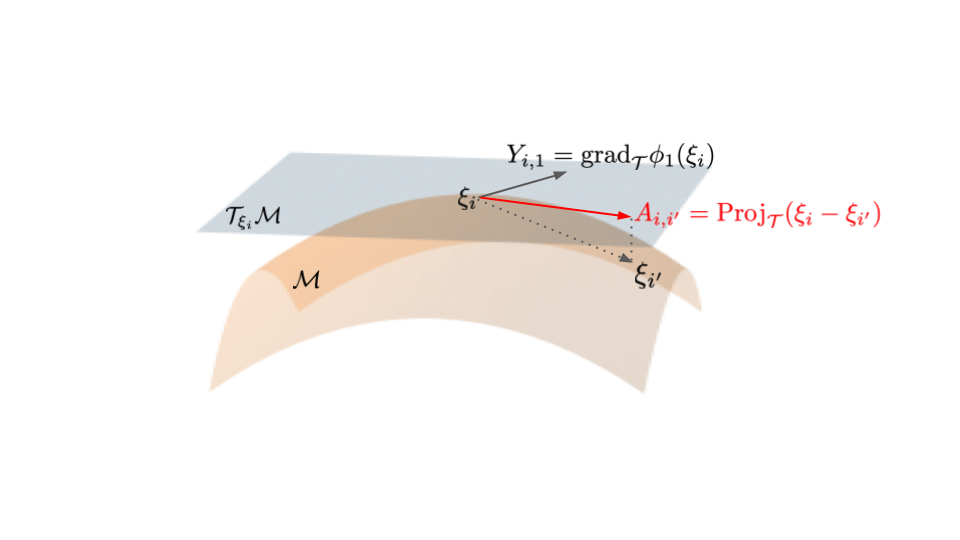
\includegraphics[width=0.48\textwidth]{../Figures/ManifoldSpace3.png}
%&
%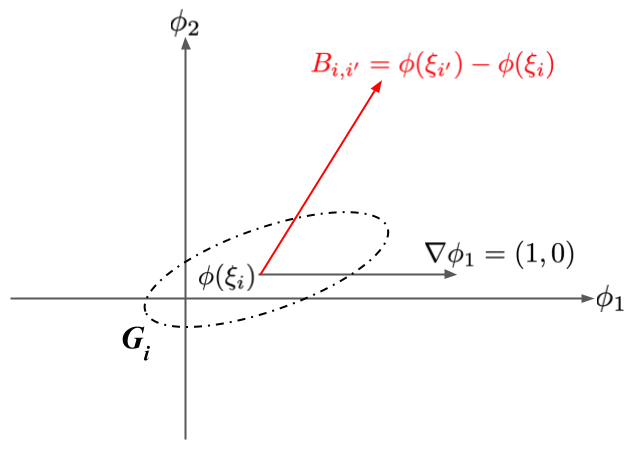
\includegraphics[width=0.48\textwidth]{../Figures/Embedded_space2.png}
%\\
%\end{tabular}
%\caption{\label{fig:pullback} Left: $\M$ with a tangent subspace at $\xi_i$, the projection $A_{i,i'}$ of $\tilde{\xi}_{i'}$ onto $\txim$ (in red), and the manifold gradient $\grad_\M\phi_1(\xi_i)$ of the first embedding coordinate $\phi_1$ (in black). The Riemannian metric on  $\M$ is the identity. Right: for $m=d=2$, $\phi(\M)$ is a (subset of) $\rrr^2$. The dotted ellipse around $\phi(\xi_i)$ represents the push-forward Riemannian metric $G_i$; in red is shown $B_{i,i'}=\phi(\xi_{i'})-\phi(\xi_i)$;  $A_{i,i'}$ is the (approximate) mapping of $B_{i,i'}$ through $D\phi^{-1}(\xi_i)$ (as in \eqref{eq:rmetric0}). The gradient $\grad_{\phi(\M)}\phi_1=\nabla \phi_1$ is trivially the first unit vector (in black). Because $(\M, \id)$ is isometric with $(\phi(\M),\g)$, the unknown $Y_{i,1}=\grad_{\txim}\phi_1$ can be obtained  from the known $A_i,B_i$ and the unit vector by solving a linear system, as in equation \eqref{eq:yi-manifold2}.}
%\end{figure}



\subsection{The \flassoalg~formulation}
\label{sec:flasso-manifold}
Recalling our assumption that $\phi=h\circ g_S$, we shall denote by
$h_k$ the $k$-th component of the vector valued function $h$.
  Recall that $X_i$ defined in
\eqref{eq:X-manifold} contains the gradients of the dictionary
functions $g_j$, and that  $y_{ik}\in \rrr^d$, the $k$-th column of $Y_i$, represents the coordinates of $\grad_{\M}\phi_k(\xi_i)$ in the chosen basis of \txim.
Further, let
%
\beq \label{eq:beta-ijk} \beta_{ijk}=\fracpartial{h_k}{g_j}( g_j( \xi_i)),
\quad \beta=[\beta_{ijk}]_{i,k,j=1}^{n,m,p}, \eeq
\beq \label{eq:betas-manifold}
\beta_j=\operatorname{vec}(\beta_{ijk},\;i=1:n,k=1:m)\in\rrr^{mn},
\quad \beta_{ik}=\operatorname{vec}(\beta_{ijk},\;j=1:p)\in\rrr^{p}.
\eeq
%
In a regression of $Y_{1:n}$ on $X_{1:n}$, $\beta_{ik}$ is the set of regression
coefficients of $y_{ik}$ onto $X_i$. Further, $\beta_j$ represents
the vector of regression coefficients corresponding to the effect of
function $g_j$, which form {\em group} $j$ in the {\em Group Lasso} \citep{Yuan2006-af}
problem defined below. The size of each group is $mn$.

We minimize the  the following objective function w.r.t. $\beta$.
%
\beq\label{eq:flasso-manifold}
J_{\lambda}(\beta)\;=\;\frac{1}{2}\sum_{i=1}^n\sum_{k=1}^m||y_{ik}-X_i\beta_{ik}||^2+\frac{\lambda}{\sqrt{mn}}\sum_{j=1}^p||\beta_j||.
\eeq
%
This is a convex optimization problem, known as the Group Lasso, introduced by \citet{Yuan2006-af}. 
The first term of the objective is the least squares loss of
regressing $Y_{1:n}$ onto $X_{1:n}$. The second is a regularization
term, which penalizes each group $\beta_j$ by its Euclidean
norm. Note that $||\beta_j||$ encourages most $\beta_j$ groups to be
identically 0. The normalization of the regularization coefficient
$\lambda$ by the group size $mn$ follows \citet{Yuan2006-af}. 

The use of Group Lasso for sparse functional regression was introduced in \citet{MKoelleZhang:arxiv1811-11891}, where recovery conditions for the objective function \eqref{eq:flasso-manifold} are given.

Note that $J_\lambda(\beta)$ is invariant to the change of basis
$T_i$. Let $\tilde{T}_i=T_i\Gamma$ be a different basis, with
$\Gamma\in \rrr^{d\times d}$ a unitary matrix. Then,
$\tilde{y}_{ik}=\Gamma^Ty_{ik}$, $\tilde{X}_i=\Gamma^TX_i$, and
$||\tilde{y}_{ik}-\tilde{X}_i\beta||^2=||y_{ik}-X_i\beta||^2$.

\subsection{Computation, normalization, and tuning}
\paragraph{Computation}
\label{sec:ouralg-computation}
The first two steps of \ouralg~are construction of the neighborhood
graph and estimation of the Laplacian $L$. As shown in Section
\ref{sec:background}, $L$ is a sparse matrix, hence \rmalg~can be run
efficiently by only passing values corresponding to one neighborhood
at a time. Note that in our examples and experiments, Diffusion Maps
is our chosen embedding algorithm, so the neighborhoods and Laplacian are already available, though in general this is not the case.

The second part of the algorithm estimates the gradients and
constructs matrices $Y_{1:n},X_{1:n}$.  The gradient estimation
runtime is $O(qd^2 + nd^3)$ where $q$ is the number of edges in the
neighborhood graph, using Cholesky decomposition-based
solvers. Finally, the last step is a call to the \glassoalg, which
estimates the support $S$ of $\phi$. The computation time of each
iteration in \glassoalg~is $O(n^2 m^2 pd)$.  For large data sets, one
can perform the ``for'' loop over a subset $\I\subset[n]$ of the
original data while retaining the geometric information from the full
data set. This replaces the $n$ in the computation time with the
smaller factor $|\I|$.

\paragraph{Normalization}
\label{sec:ouralg-normalization}
Multiplying $g_j$ by a non-zero constant and dividing
its corresponding $\beta_j$ by the same constant leaves the
reconstruction error of all $y$'s invariant, but affects the norm
$||\beta_j||$. Therefore, the relative scaling of the dictionary
functions $g_j$ can influence the recovered support $S$, by favoring
the dictionary functions whose columns have larger norm.

We therefore follow \citet{Haufe2009-yt} in normalizing all columns of the regression matrix to 1. When the dictionary functions $g_j$ are defined on $\M$, but not
outside $\M$, we calculate the {\em normalizing constant}
\beq \label{eq:gammaj-discrete-M}
\gamma_j^2\;=\;\frac{1}{n}\sum_{i=1}^n\|\grad_{T_i} g_j(\xi_i)||^2;
\eeq
%
then we set $g_j\leftarrow g_j/\gamma_j$.  The above $\gamma_j$ is the
finite sample version of $\|\grad_\T g_j\|_{L_2(\M)}$, integrated
w.r.t. the data density on $\M$.

When the dictionary functions are defined on a neighborhood around $\M$ in $\rrr^D$, we compute the normalizing constant with respect to  $\nabla_\xi g_j$. That is,
\beq \label{eq:gammaj-discrete-xi}
\gamma_j^2\;=\;\frac{1}{n}\sum_{i=1}^n\| \nabla_\xi g_j(\xi_i)\|^2.
\eeq
Then, once again, we set $g_j\leftarrow g_j/\gamma_j$. Doing this favors dictionary functions whose gradients are tangent to the manifold $\M$, and penalizes the $g_j$'s which have large gradient components perpindicular to $\M$.

\paragraph{Tuning}
\comment{ 1a sentence on the effect of lambda: large$=$ smaller support,
  etc, 2. for single chart, .... 3. for multiple charts s at least
  d. 4. shall we talk about this or not? in standard lasso cv; we are
  considering it too.  } 
 As the tuning parameter $\lambda$ is
increased, the cardinality of the support decreases.  Tuning
parameters are often selected by cross-validation in Lasso-type
problems, but this is not possible in our unsupervised setting. We
base our choice of $\lambda$ on matching the cardinality of the
support to $d$. In Section 
\ref{sec:theory}, we give sufficient conditions for when $s=d$.

\comment{
However, one can also accept $s>d$
when functions are coherent, like when a dihedral angle has multiple
equivalent formulations, or when no single dictionary function can
parametrize the manifold, like when $\phi$ has piecewise functional
support. A recursive procedure, in which functions discovered to be in
the support are removed from the dictionary and the algorithm is rerun
to uncover dependencies on remaining functions, could also be
used.
}

\comment{In manifolds which cannot be represented by a single chart, the
situation is more complicated, depending on the topology of the
co-domains of the functions $g_j$, and also the quality of the dictionary. For example, in the toluene data
presented in Section \ref{sec:exps}, the manifold is a
circle. This cannot be covered by a single chart, but it can be
parametrized by a single function in the dictionary, the angle of the
bond torsion in Figure \ref{fig:mds-toluene} since the discontinuity of the dictionary function is only at a point of measure zero; hence $s=d$.  The case $s>d$ occurs
when no single dictionary function can parametrize the manifold. For example, when $\M$ is a circle in the plane $(\xi_1,\xi_2)$ and the dictionary consists of the coordinate functions, i.e. $\G=\{g_1\equiv \xi_1,g_2\equiv \xi_2\}$, neither dictionary function can explain $\M$ globally.  Furthermore, when
$\G$ is not a functionally independent set, it is possible that the
parametrization of $\M$ by $\G$ is not unique. In this case, the minimizer of $J_\lambda$ in equation \eqref{eq:flasso-manifold} will be one of the possible support sets $S$.}

\subsection{Variants and extensions}
The approach utilized here can be extended in several interesting
ways. First, our current approach explains the embedding coordinates
$\phi$ produced by a particular embedding algorithm. However, the same
approach can be used to directly explain the tangent subspace of $\M$,
independently of any embedding.

Second, one could set up \flassoalg~problems that explain a single
coordinate function.  In general, manifold coordinates do not have
individual meaning, so it will not always be possible to find a good
explanation for a single $\phi_k$.  However, Figure \ref{fig:mds-ethanol} shows
that for the ethanol molecule, whose manifold is a torus, there exists
a canonical system of coordinates in which each coordinate is
explained by one torsion.

Third, in future work, we plan to examine more closely cases such as the above. It is known \citep{AbrahamMarsden} that Hamiltonian systems are associated with tori; hence, it is natural to consider dictionaries of functions $g:\M\rightarrow S^1$.

\comment{\mmp{what is this?}Fourth, the pushforward metric associated with each of
the individual functional covariates can be estimated with respect to
the data. This enables estimation of sparse functional support that is
more robust to curvature than our current approach, , where the
codomain of $g_j$ is assumed to have identity metric, and is analogous
to finding a flat parameterization of $\M$. Normalization is
equivalent to saying that the metric on the codomain of the dictionary
functions is unknown by a constant factor, while the definition of
norm we use assumes that the metric on the codomain cancels out the
metric on $\phi(\M)$.}  \mmp{don't comment with \%. When no more
  needed, just delete. We have all the previous version if we want
  them.  and regularization here?// project or don't project
  gradients?// Step Embedding can be substituted with any other
  embedding algorithm. To lift $Y_i$ in $\rrr^D$, set $Y_i\leftarrow
  T_iY_i$.  }


